\documentclass[12pt, a4paper, oneside]{ctexart}
\usepackage{amsmath, amsthm, amssymb, bm, color, graphicx, geometry, mathrsfs,extarrows, braket, booktabs, array, wrapfig}
\usepackage[colorlinks,linkcolor=red,anchorcolor=blue,citecolor=blue,urlcolor=blue,menucolor=black]{hyperref}
\setCJKmainfont{方正新书宋_GBK.ttf}[ BoldFont = 方正小标宋_GBK, ItalicFont = 方正楷体_GBK]
\setmainfont{Times New Roman}  % 设置英文字体
\setsansfont{Calibri}
\setmonofont{Consolas}

\linespread{1.4}
%\geometry{left=2.54cm,right=2.54cm,top=3.18cm,bottom=3.18cm}
\geometry{left=1.84cm,right=1.84cm,top=2.18cm,bottom=2.18cm}
\newcounter{problem}  % 问题序号计数器
\newenvironment{problem}[1][]{\stepcounter{problem}\par\noindent\textbf{题目\arabic{problem}. #1}}{\smallskip\par}
\newenvironment{solution}[1][]{\par\noindent\textbf{#1解答. }}{\smallskip\par}  % 可带一个参数表示题号\begin{solution}{题号}
\newenvironment{note}{\par\noindent\textbf{注记. }}{\smallskip\par}

%%%% 图片相对路径 %%%%
\graphicspath{{figure/}} % 当前目录下的figure文件夹, {../figure/}则是父目录的figure文件夹

\everymath{\displaystyle} % 默认全部行间公式
\DeclareMathOperator*\uplim{\overline{lim}} % 定义上极限 \uplim_{}
\DeclareMathOperator*\lowlim{\underline{lim}} % 定义下极限 \lowlim_{}
\let\leq=\leqslant % 将全部leq变为leqslant
\let\geq=\geqslant % geq同理

%%%% 一些宏定义 %%%%
\def\bd{\boldsymbol}        % 加粗(向量) boldsymbol
\def\disp{\displaystyle}    % 使用行间公式 displaystyle(默认)
\def\tsty{\textstyle}       % 使用行内公式 textstyle
\def\sign{\text{sign}}      % sign function
\def\wtd{\widetilde}        % 宽波浪线 widetilde
\def\R{\mathbb{R}}          % Real number
\def\N{\mathbb{N}}          % Natural number
\def\Z{\mathbb{Z}}          % Integer number
\def\Q{\mathbb{Q}}          % Rational number
\def\C{\mathbb{C}}          % Complex number
\def\K{\mathbb{K}}          % Number Field
\def\P{\mathbb{P}}          % Polynomial
\def\d{\mathrm{d}}          % differential operator
\def\e{\mathrm{e}}          % Euler's number
\def\i{\mathrm{i}}          % imaginary number
\def\re{\mathrm{Re}}        % Real part
\def\im{\mathrm{Im}}        % Imaginary part
\def\res{\mathrm{Res}}      % Residue
\def\L{\mathcal{L}}         % Loss function
\def\wdh{\widehat}          % 宽帽子 widehat
\def\ol{\overline}          % 上横线 overline
\def\ul{\underline}         % 下横线 underline
\def\add{\vspace{1ex}}      % 增加行间距
\def\del{\vspace{-1.5ex}}   % 减少行间距

%%%% 定理类环境的定义 %%%%
\newtheorem{theorem}{定理}

%%%% 基本信息 %%%%
\newcommand{\RQ}{\today} % 日期
\newcommand{\km}{泛函分析} % 科目
\newcommand{\bj}{强基数学002} % 班级
\newcommand{\xm}{吴天阳} % 姓名
\newcommand{\xh}{2204210460} % 学号

\begin{document}

%\pagestyle{empty}
\pagestyle{plain}
\vspace*{-15ex}
\centerline{\begin{tabular}{*5{c}}
    \parbox[t]{0.25\linewidth}{\begin{center}\textbf{日期}\\ \large \textcolor{blue}{\RQ}\end{center}} 
    & \parbox[t]{0.2\linewidth}{\begin{center}\textbf{科目}\\ \large \textcolor{blue}{\km}\end{center}}
    & \parbox[t]{0.2\linewidth}{\begin{center}\textbf{班级}\\ \large \textcolor{blue}{\bj}\end{center}}
    & \parbox[t]{0.1\linewidth}{\begin{center}\textbf{姓名}\\ \large \textcolor{blue}{\xm}\end{center}}
    & \parbox[t]{0.15\linewidth}{\begin{center}\textbf{学号}\\ \large \textcolor{blue}{\xh}\end{center}} \\ \hline
\end{tabular}}
\begin{center}
    \zihao{-3}\textbf{第五次作业}
\end{center}
\vspace{-0.2cm}
% 正文部分
\begin{problem}[(1.4.1)]
    在二维空间$\R^2$中,对每一点$z=(x,y)$,令
    \begin{equation*}
        ||z||_1=|x|+|y|;\quad ||z||_2=\sqrt{x^2+y^2};\quad ||z||_3=\max(|x|,|y|);\quad ||z||_4=(x^4+y^4)^{\frac{1}{2}}.
    \end{equation*}

    (1) 求证$||\cdot||_i\ (i=1,2,3,4)$都是$\R^2$的范数.

    (2) 画出$(\R^2,||\cdot ||_i)\ (i=1,2,3,4)$各空间中的单位球面图形.

    (3) 在$\R^2$中取定三点$O=(0,0),\ A=(1,0),\ B=(0,1)$,试在上述四种不同范数下求出$\triangle OAB$三边的长度.
\end{problem}
\begin{solution}
    (1). $\forall x, y\in \R^2$,令$x = (x_1,x_2),\ y=(y_1,y_2)$.
    
    正定性:由于$|x_1|,x_1^2,x_1^4\geq 0$,则$||x||_i\geq 0,\ (i=1,2,3,4)$且$||x||_i=0\iff x=(0,0),\ (i=1,2,3,4)$.

    三角不等式:$||x+y||_1=|x_1+y_1|+|x_2+y_2|\leq |x_1|+|x_2|+|y_1|+|y_2|=||x||_1+||y||_1$.

    下证p-范数上的三角不等式,$||x||_p = \left(|x_1|^p+|x_2|^p\right)^{\frac{1}{p}}$
    \begin{align*}
        ||x+y||_p^p =&\ \sum_{i=1}^2|x_i+y_i|^{p-1}|x_i+y_1|\leq \sum_{i=1}^2|x_i|\cdot|x_i+y_i|^{p-1}+\sum_{i=1}^2|y_i|\cdot |x_i-y_i|^{p-1}\\
        \text{(Holder不等式)}\leq&\ \left(\left(\sum_{i=1}^2|x_i|^p\right)^{\frac{1}{p}}+\left(\sum_{i=1}^2|y_i|^p\right)^{\frac{1}{p}}\right)\left(\sum_{i=1}^2|x_i+y_i|^p\right)^{\frac{p-1}{p}} = (||x||_p+||y||_p)||x+y||_p^{p-1}
    \end{align*}
    则$||x+y||_p\leq ||x||_p+||y||_p$,故$||\cdot||_2,\ ||\cdot||_4$满足三角不等式.

    $||x+y||_3 = \max(|x_1+y_1|,|x_2+y_2|)\leq \max(|x_1|+|y_1|,|x_2|+|y_2|)\leq \max(|x_1|,|x_2|)+\max(|y_1|,|y_2|) = ||x||_3+||y||_3$.

    齐次型:$\forall \alpha \in \K$,由于$|\alpha x_1| = |\alpha|\cdot |x_1|,\ \sqrt{\alpha^2} = (\alpha^4)^{\frac{1}{4}}=|\alpha|$,则以上范数均满足齐次性.

\begin{wrapfigure}[20]{r}{.4\linewidth} % 文字环绕行数为13行, 图片靠右 (l为靠左), 图片占0.5的行宽
    \centering
    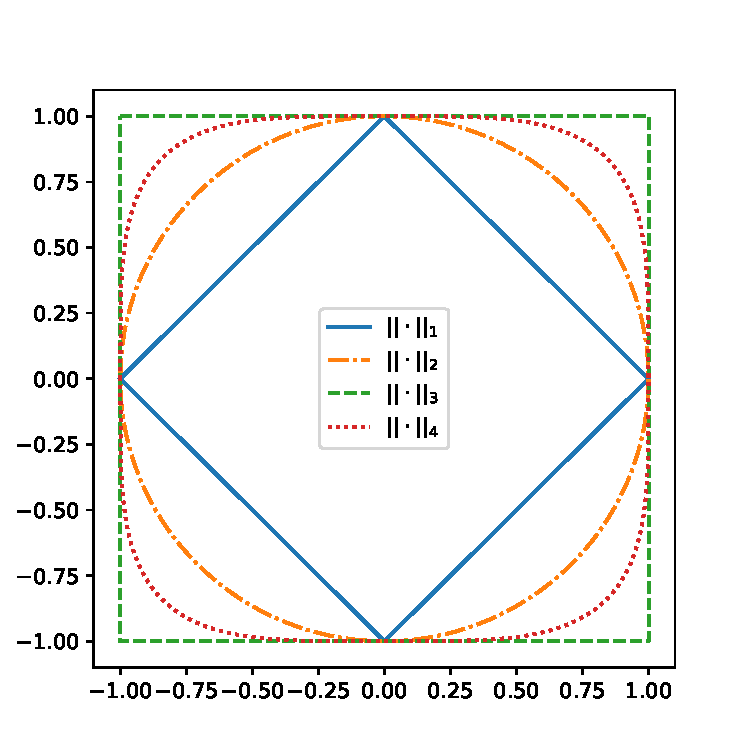
\includegraphics[scale=0.7]{1.4.1.pdf} % scale=0.7按比例缩放70%
\end{wrapfigure}
    (2). 单位球面如右图所示

    (3). $||OA||_i = ||OB||_i = ||(1,0)||_1 = ||(0,1)||_1 = 1$.
    
    $||AB||_1=2,\ ||AB||_2=\sqrt{2},\ ||AB||_3=1,\ ||AB||_4=2^{\frac{1}{4}}$.
\end{solution}
\begin{problem}[(1.4.3)]
    在$C^1[a,b]$中,令\add
    \begin{equation*}
        \hspace*{-8cm}||f||_1=\left(\int_a^b(|f|^2+|f'|^2)\,\d x\right)^{\frac{1}{2}},\quad(\forall f\in C^1[a,b]),
    \end{equation*}

    (1) 求证$||\cdot ||_1$是$C^1[a,b]$上的范数.

    (2) 问$(C^1[a,b],||\cdot||_1)$是否完备?
\end{problem}
\begin{solution}
    由定义易得$||f||\geq 0$,当$f\equiv 0$时,$||f||=0$,\\反之,当$||f|| = 0$时,
    \begin{equation*}
        \int_a^b(|f|^2+|f'|^2)\,\d x = 0\Rightarrow |f|^2\text{在}[a,b]\text{上几乎处处为0}   
    \end{equation*}
    由于$f\in C[a,b]$,则$f\equiv 0$.

    三角不等式:\begin{align*}\hspace*{-1cm}
        ||f+g||^2 =&\ \int_a^b\left(|f+g|^2+|f'+g'|^2\right)\,\d x\leq \int_a^b \left(|f|\cdot|f+g|+|f'|\cdot|f'+g'|+|g|\cdot|f+g|+|g'|\cdot|f'+g'|\right)\,\d x\\
        \leq&\ \int_a^b\left(\sqrt{|f|^2+|f'|^2}\sqrt{|f+g|^2+|f'+g'|^2}+\sqrt{|g|^2+|g'|^2}\sqrt{|f+g|^2+|f'+g'|^2}\right)\,\d x\\
        \leq&\ \left(\int_a^b(|f|^2+|f'|)\,\d x\right)^{\frac{1}{2}}\left(\int_a^b(|f+g|^2+|f'+g'|^2)\,\d x\right)^{\frac{1}{2}}\\
        &\ +\left(\int_a^b(|g|^2+|g'|^2)\,\d x\right)^{\frac{1}{2}}\left(\int_a^b(|f+g|^2+|f'+g'|^2)\,\d x\right)^{\frac{1}{2}}\,\d x\\
        =&\ (||f||+||g||)\,||f+g||
    \end{align*}
    则$||f+g||\leq ||f||+||g||$.

    齐次性:$\forall \alpha \in \K$,则$||\alpha f|| = \int_a^b(|\alpha f|^2+|\alpha f'|^2)\,\d x= |\alpha|\int_a^b(|f|^2+|f'|^2)\,\d x = |\alpha|\cdot||f||$.

    (2) 不完备. 令$\varphi_n(x) = \left(\frac{x-a}{b-a}\right)^{\frac{1}{n}}$,则$\{\varphi_n\}\subset C^1[a,b]$,令$\varphi(x) = \begin{cases}
        0,&\quad x=a,\\ 1,&\quad a<x\leq b.
    \end{cases}$下证$\varphi_n\to \varphi$.
    \begin{align*}
        ||\varphi_n-\varphi||^2 =&\ \int_a^b\left\{\left(\left(\frac{x-a}{b-a}\right)^{\frac{1}{n}}-1\right)^2+\left(\frac{1}{n}\left(\frac{x-a}{b-a}\right)^{\frac{1-n}{n}}\right)^2\right\}\,\d x\\
        =&\ \int_a^b\left(\frac{x-a}{b-a}\right)^{\frac{2}{n}}\,\d x - 2\int_a^b\left(\frac{x-a}{b-a}\right)^{\frac{1}{n}}\,\d x+\int_a^b\,\d x + \frac{1}{n^2}\int_a^b\left(\frac{x-a}{b-a}\right)^{\frac{2-2n}{n}}\,\d x\\
        =&\ \frac{b-a}{\frac{2}{n}+1}-\frac{2(b-a)}{\frac{1}{n}+1}+b-a+\frac{1}{n^2\left(\frac{2-2n}{n}+1\right)}\to b-a-2(b-a)+b-a=0,\quad (n\to\infty).
    \end{align*}
    则$\varphi_n\to\varphi,\ (n\to\infty)$,而$\varphi\notin C^1[a,b]$,则$(C^1[a,b],||\cdot||)$不完备.
\end{solution}
\begin{problem}[(1.4.4)]
    在$C[0,1]$中,对每一个$f\in C[0,1]$,令
    \begin{equation*}
        ||f||_1=\left(\int_0^1|f|^2\,\d x\right)^{\frac{1}{2}},\quad ||f||_2=\left(\int_0^1(1+x)|f|^2\,\d x\right)^{\frac{1}{2}},
    \end{equation*}
    求证:$||\cdot ||_1$和$||\cdot ||_2$是$C[0,1]$中的两个相等范数.
\end{problem}
\begin{proof}
    由于$x\in [0,1]$时
    \begin{equation*}
        \left(\int_0^1|f|^2\,\d x\right)^{\frac{1}{2}}\leq \left(\int_0^1(1+x)|f|^2\,\d x\right)^{\frac{1}{2}}\leq \left(\int_0^1 2|f|^2\,\d x\right)^{\frac{1}{2}}=\sqrt{2}\left(\int_0^1|f|^2\,\d x\right)^{\frac{1}{2}}.
    \end{equation*}
    所以$||\cdot ||_1$与$||\cdot ||_2$等价.
\end{proof}
\begin{problem}[(1.4.6)]
    设$BC[0,\infty]$表示$[0,\infty)$上连续且有界的函数$f(x)$全体,对于每个$f\in BC[0,\infty)$及$a>0$,定义
    \begin{equation*}
        ||f||_a=\left(\int_0^\infty \e^{-ax}|f|^2\,\d x\right)^{\frac{1}{2}}.
    \end{equation*}

    (1) 求证$|\cdot ||_a$是$BC[0,\infty)$上的范数.

    (2) 若$a,b > 0,\ a\neq b$,求证$||\cdot ||_a$与$||\cdot ||_b$作为$BC[0,\infty)$上的范数是不等价的.
\end{problem}
\begin{proof}
    先证明定义$||\cdot ||_a$有意义,$\forall f\in BC[0,\infty)$,设$\sup_{x\geq 0}|f(x)| = M$,则
    \begin{equation*}
    ||f||_a=\left(\int_0^\infty \e^{-ax}|f|^2\,\d x\right)^{\frac{1}{2}}\leq |M|\left(\int_0^\infty \e^{-ax}\,\d x\right)^{\frac{1}{2}}=\frac{|M|}{\sqrt{a}}.
    \end{equation*}

    再证明$||\cdot ||_a$满足范数定义. 正定性:由于$|f|^2\geq 0$,则$||f||_a\geq 0$,当$f\equiv 0$时,$||f||_a = 0$,反之,当$||f||_a=0$时,$|f|^2$在$[0,\infty)$上几乎处处为零,又由于$f\in C[0,\infty)$,则$f\equiv 0$.

    三角不等式:
    \begin{align*}
        ||f+g||_a^2 =&\ \int_0^{\infty}\e^{-ax}|f+g|^2\,\d x = \int_0^{\infty}\e^{-\frac{ax}{2}}|f|\cdot \e^{-\frac{ax}{2}}|f+g|\,\d x+\int_0^{\infty}\e^{-\frac{ax}{2}}|g|\cdot \e^{-\frac{ax}{2}}|f+g|\,\d x\\
        \leq&\ \left(\int_0^\infty \e^{-ax}|f|^2\,\d x\right)^{\frac{1}{2}}\left(\int_0^{\infty}\e^{-ax}|f+g|^2\,\d x\right)^{\frac{1}{2}}+\left(\int_0^\infty \e^{-ax}|g|^2\,\d x\right)^{\frac{1}{2}}\left(\int_0^{\infty}\e^{-ax}|f+g|^2\,\d x\right)^{\frac{1}{2}}\\
        =&\ (||f||_a+||g||_a)\,||f+g||_a,
    \end{align*}
    则$||f+g||_a\leq ||f||_a+||g||_a$.

    齐次性:$\forall \alpha \in \K$,$||\alpha f||_a=\left(\int_0^\infty \e^{-ax}|\alpha f|^2\,\d x\right)^{\frac{1}{2}}=|\alpha|\left(\int_0^\infty \e^{-ax}|f|^2\,\d x\right)^{\frac{1}{2}}=|\alpha|\cdot ||f||_a$.

    (2)
\end{proof}
\begin{problem}[(1.4.6)]
    设$X_1,X_2$是两个$B^*$空间,$x_1\in X_1$和$x_2\in X_2$的序对$(x_1,x_2)$全体构成空间$X=X_1\times X_2$,并赋以范数
    \begin{equation*}
        ||x|| = \max(||x_1||_1,||x_2||_2),
    \end{equation*}
    其中$x=(x_1,x_2),\ x_1\in X_1,\ x_2\in X_2,\ ||\cdot ||_1$和$||\cdot ||_2$分别是$X_1$和$X_2$的范数. 求证:如果$X_1,X_2$是$B$空间,那么$X$也是$B$空间.
\end{problem}
\begin{proof}
    令$\{x_n\}\subset X$是Cauchy列,则$||x_n-x_m||\to 0,\ (n,m\to 0)$,令$x_n = (x_1^{(n)}, x_2^{(n)})$,则
    \begin{equation*}
        \max\left(||x_1^{(n)}-x_1^{(m)}||_1,||x_2^{(n)}-x_2^{(m)}||_2\right)\to 0,\quad (n,m\to 0)
    \end{equation*}
    则$||x_i^{(n)}-x_i^{(m)}||_i\to 0,\ (n,m\to\infty,\ i=1,2)$,由于$X_1,X_2$是$B$空间,则$\exists x_1^{(0)}\in X_1,\ x_2^{(0)}\in X_2$使得$||x_i^{(n)}-x_i^{(0)}||_i\to 0,\ (n\to\infty,\ i=1,2)$,令$x_0 = (x_1^{(0)}, x_2^{(0)})$,则
    \begin{equation*}
        ||x_n-x_0|| = \max(||x_i^{(n)}-x_1^{(0)}||, ||x_2^{(n)}-x_2^{(0)})\to 0,\quad(n\to \infty)
    \end{equation*}
    所以$\{x_n\}$收敛于$x_0$,故$X$是$B$空间.
\end{proof}
\begin{problem}[(1.4.8)]
    记$[a,b]$上次数不超过$n$的多项式全体为$\P_n$. 求证:$\forall f(x) \in C[a,b],\ \exists P_0(x)\in \P_n$使得
    \begin{equation*}
        \max_{a\leq x\leq b}|f(x)-P_0(x)| = \min_{P\in \P_n}\max_{a\leq x\leq b}|f(x)-P(x)|.
    \end{equation*}
    也就是说,如果用所有次数不超过$n$的多项式去对$f(x)$一致逼近,那么$P_0(x)$是最佳的.
\end{problem}
\begin{proof}
    令$C[a,b]$上的范数为$||f|| = \max_{a\leq x\leq b}|f(x)|$则$(C[a,b], ||\cdot||)$是$B^*$空间. 由于$\P_n$是$C[a,b]$的真闭子空间且$\dim \P_n = n+1 < \infty$,则存在最佳逼近,即$\forall f\in C[a,b],\ \exists P_0\in \P_n$使得$||f-P_0||=\rho(f,\P_n)$,也即
    \begin{equation*}
        \max_{a\leq x\leq b}|f(x)-P_0(x)| = \min_{P\in \P_n}\max_{a\leq x\leq b}|f(x)-P(x)|.
    \end{equation*}
\end{proof}
\begin{problem}[(1.4.9)]
    在$\R^2$中,对$\forall x = (x_1,x_2)\in \R^2$,定义范数
    \begin{equation*}
        ||x|| = \max(|x_1|,|x_2|),
    \end{equation*}
    并设$e_1=(1,0),\ x_0=(0,1)$. 求$a\in \R$使得
    \begin{equation*}
        ||x_0-ae_1||=\min_{\lambda\in \R}||x_0-\lambda e_1||,
    \end{equation*}
    并问这样的$a$是否唯一?请对结果做出几何解释.
\end{problem}
\begin{solution}
    不唯一. $||x_0-\lambda e_1|| = ||(-\lambda ,1)|| = \max(|\lambda|, 1)\geq 1$当$|\lambda|\leq 1$时取到最小值$1$. 则$a\in [-1,1]$.
    
    若把$\{\lambda e_1:\lambda\in \R$视为一维平面,则$x_0$到该平面的投影不唯一.
\end{solution}
\begin{problem}[(1.4.10)]
    求证:范数的严格凸性等价于下列条件:
    \begin{equation*}
        ||x+y||=||x||+||y|\ (\forall x\neq 0, y\neq 0)\Rightarrow x=cy\quad (c > 0).
    \end{equation*}
\end{problem}
\begin{proof}
    充分性,证明其逆否命题. $\forall x, y\neq \theta$,$x\neq cy\ (c > 0)$,只需证$||x+y|| < ||x||+||y||$,不妨令$||x||\geq ||y||$.

    (i) 当$||x|| = ||y||=:d$时,$\left|\left|\frac{1}{2}\frac{x}{d}+\frac{1}{2}\frac{y}{d}\right|\right| < \frac{1}{2}+\frac{1}{2}\Rightarrow ||x+y|| < d+d = ||x||+||y||$.\add

    (ii) 当$||x||\neq ||y||$时,不妨令$||x|| > ||y||$则
    \begin{equation*}
        \left|\left|\frac{x}{||x||}+\frac{y}{||x||}\right|\right|-\frac{||y||}{||x||}\leq \left|\left|\frac{x}{||x||}+\frac{y}{||x||}-\frac{||y||}{||x||}\right|\right|\leq \left|\left|\frac{||x||-||y||}{||x||}\frac{x}{||x||}+\frac{||y||}{||x||}\frac{y}{||y||}\right|\right|<1
    \end{equation*}
    左侧不等号是因为$||x||= ||x-y+y||\leq ||x-y||+||y||$,所以$||x||-||y||\leq ||x-y||$,于是
    \begin{equation*}
        \left|\left|\frac{x}{||x||}+\frac{y}{||x||}\right|\right| < 1+\frac{||y||}{||x||}\Rightarrow ||x+y|| < ||x||+||y||
    \end{equation*}

    必要性,反设$||\alpha x+\beta y|| = 1 = \alpha||x||+\beta||y||$,则$\exists c > 0$使得$x=cy$,由于$1=||x||=c||y|| = c$,则$x=y$矛盾.
\end{proof}
\begin{proof}[(1.4.13)]
    
\end{proof}

% 下面给一些功能的写法
\iffalse
% 图片模板
\centerline{
    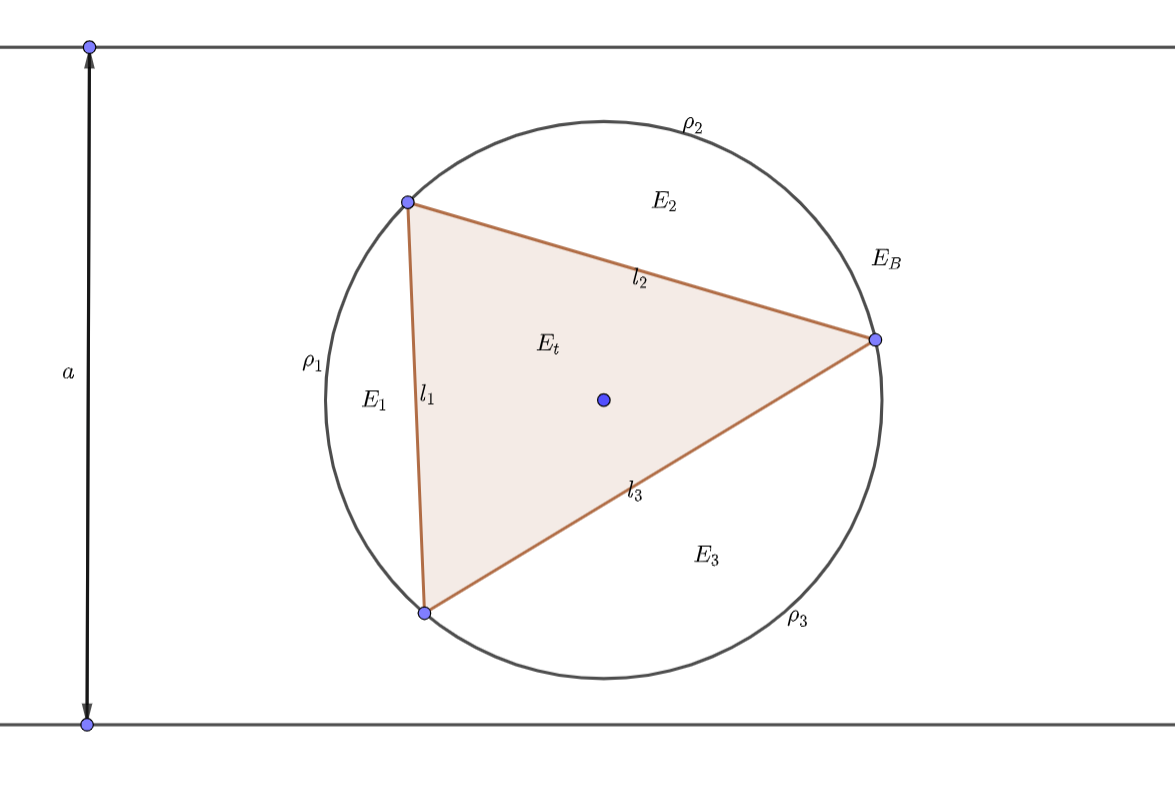
\includegraphics[width=0.8\textwidth]{figure.png}
}
% 表格模板
\renewcommand\arraystretch{0.8} % 设置表格高度为原来的0.8倍
\begin{table}[!htbp] % table标准
    \centering % 表格居中
    \begin{tabular}{p{1cm}<{\centering}p{1cm}<{\centering}p{3cm}<{\centering}p{5cm}<{\centering}} % 设置表格宽度
    %\begin{tabular}{cccc}
        \toprule
        $x_i$ & $f[x_1]$ & $f[x_i,x_{i+1}]$ & $f[x_i,x_{i+1},x_{i+2}]$ \\
        \midrule
        $x_0$ & $f(x_0)$ &                  &                          \\
        $x_0$ & $f(x_0)$ & $f'(x_0)$        &                          \\
        $x_0$ & $f(x_1)$ & $\frac{f(x_1)-f(x_0)}{x_1-x_0}$ & $\frac{f(x_1)-f(x_0)}{(x_1-x_0)^2}-\frac{f'(x_0)}{x_1-x_0}$\\
        \bottomrule
    \end{tabular}
\end{table}

\def\Log{\text{Log}} % 一个简单的宏定义
$\Log$ % 调用方法
\fi

\end{document}